Auf den Container wirken zwei Kräfte: seine Gewichtskraft $m\,g$ nach unten und die Seilkraft $\ssc{F}{S}$ nach oben. Die Beschleunigung zeigt nach oben:
\begin{align}
 \ssc{F}{S} - m\,g &= m\,a
\end{align}

\begin{center}
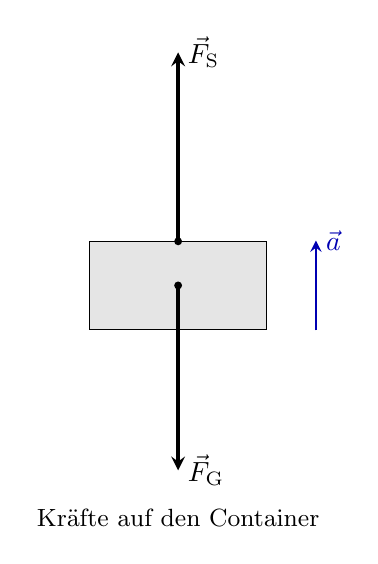
\begin{tikzpicture}[>=stealth]
 \draw[fill=gray!20] (-1.12,-0.56) rectangle (1.12,0.56);
 \draw[->, very thick] (0,0.56) -- (0,2.96);
 \fill (0,0.56) circle (0.05);
 \node[right] at (0,2.96) {$\vec F_\mathrm{S}$};
 \draw[->, very thick] (0,0) -- (0,-2.35);
 \fill (0,0) circle (0.05);
 \node[right] at (0,-2.35) {$\vec F_\mathrm{G}$};
 \draw[->, thick, blue!70!black] (1.75,-0.57) -- (1.75,0.57) node[right] {$\vec a$};
 \node[font=\small] at (0,-2.95) {Kräfte auf den Container};
\end{tikzpicture}
\end{center}

\begin{abcliste}
\abc
\begin{align}
 \ssc{F}{S} &= \FSF \\
   &= \mC\cdot(\g+\a) \\
   &= \FS \approx \result{\FSP{3}{3}}
\end{align}

\abc
An der Grenze des Seils ist $\ssc{F}{S} = \ssc{F}{max}$:
\begin{align}
 \ssc{a}{max} &= \amaxF \\
   &= \frac{\Fmax-\mC\cdot\g}{\mC} \\
   &= \amax \approx \result{\amaxP{0}{2}}
\end{align}
Das meiste, was das Seil tragen kann, braucht es, um den Container zu halten.
\end{abcliste}
